% CS229 Project Milestone
\documentclass{article}

\usepackage[preprint,nonatbib]{cs229}
\usepackage[utf8]{inputenc}
\usepackage[T1]{fontenc}
\usepackage{lmodern}  % Type-1 Latin Modern, avoids missing-bitmap-font errors with [T1]{fontenc} on minimal TeX installs
\usepackage{hyperref}
\usepackage{url}
\usepackage{booktabs}
\usepackage{amsfonts}
\usepackage{microtype}
\usepackage{xcolor}
\usepackage{amsmath}
\usepackage{fancyhdr}
\usepackage{graphicx}
\usepackage{caption}

\pagestyle{fancy}
\fancyhf{}
\fancyhead[C]{CS229 Project Milestone}
\renewcommand{\headrulewidth}{0.4pt}

\renewcommand{\maketitle}{
  \begin{center}
    {\bf \large Micro-Transformer: A From-Scratch Autograd and Attention Engine for Character-Level Language Modeling}\\
    \vspace{0.1cm}
    {\bf Team Members:} Manikanta Harsha Nadimpalli, Luis Blanco Hoyos\\
    \vspace{0.1cm}
    {\bf Emails (SUNet):} nmharsha@stanford.edu, blancol@stanford.edu\\
    \vspace{0.2cm}
  \end{center}
}

\begin{document}

\maketitle

\section{Motivation}
We are building a reverse-mode autograd engine and a small transformer~\cite{vaswani2017attention} on top of it from scratch in NumPy, with one specific scientific question in mind: \emph{how do LayerNorm~\cite{ba2016layernorm} placement (pre-norm, post-norm, none) and residual connections shape the gradient signal that reaches the early layers of a decoder-only transformer during training on character-level language modeling?} The from-scratch build is the instrument; the gradient-flow ablation is the contribution. Existing frameworks expose hooks and functional Jacobians, but constructing the engine ourselves gives us conceptual clarity over every chain-rule edge and exact, low-overhead access to per-layer activation and gradient statistics, with no framework internals to reverse-engineer.

The milestone deliverables described below are the foundation of that instrument: a data pipeline, three classical baselines, a scalar reverse-mode engine, a tensor reverse-mode engine with the full op surface needed for an MLP, and a first non-trivial language model trained end-to-end through our own engine. The ablation grid itself is post-milestone work and tracked under \emph{Next Steps}.

\section{Methods}

\subsection{Data and tokenization} Tiny Shakespeare~\cite{karpathy2015charrnn} (1{,}115{,}394 characters, 65 unique symbols), char-level tokenization. Train/val split is 90/10 \emph{by position}, not random; random char-level shuffling would leak local context across the boundary and inflate val performance. Sampling uses caller-supplied \texttt{np.random.Generator} so every run is reproducible at the seed.

\subsection{Baselines (closed-form and SGD)} Three reference points anchor every later result:
\begin{itemize}
\setlength{\itemsep}{0pt}
  \item \textbf{Uniform predictor.} Cross-entropy floor of $\log V$ nats.
  \item \textbf{Closed-form bigram} with Laplace smoothing ($\alpha\!=\!1$). Direct count $\to$ normalize on train. Smoothing is required because val contains bigrams unseen in train.
  \item \textbf{Softmax regression by SGD.} The same model class as the bigram (logits $= W[i] + b$) trained by mini-batch SGD with hand-derived gradients in plain NumPy. Convergence behavior under SGD is itself a sanity check: the SGD trajectory should approach the closed-form CE.
\end{itemize}

\subsection{Scalar reverse-mode autograd} A Karpathy-style~\cite{karpathy2020micrograd} \texttt{Value} class wrapping a Python float. Eight elementary ops (\texttt{+}, \texttt{*}, \texttt{**}, \texttt{relu}, \texttt{tanh}, \texttt{exp}, \texttt{log}, neg/sub/div as compositions). Each forward op installs a closure that captures \texttt{(self, other, out)} and pushes the upstream gradient through its local Jacobian; \texttt{backward()} topologically sorts from the output and walks in reverse. Verified against (i) central differences and (ii) torch.autograd to bit-identical agreement on a randomized two-layer neuron.

\subsection{Tensor reverse-mode autograd} A NumPy-backed \texttt{Tensor} class lifting the same closure pattern to batched arrays. The two genuine complications are broadcasting in backward (collapsed by an \texttt{unbroadcast} helper that sums along broadcast leading axes and size-1 dims) and lazy grad allocation. The op surface is sufficient for the MLP and forward-compatible with attention: elementwise binary/unary with broadcasting, reductions \texttt{sum}/\texttt{mean} (axis + keepdims) with grad re-broadcast, batched matmul (\texttt{@}) with leading-batch fan-in, integer-array gather (the embedding lookup, with \texttt{np.add.at} scatter-add backward), reshape, \texttt{relu}, \texttt{tanh}, numerically stable \texttt{log\_softmax}, and a fused \texttt{cross\_entropy(logits, targets)} whose backward is the closed-form $(\mathrm{softmax}-\text{onehot})/B$. Every op has a numerical-gradient-check test (the non-negotiable Week 2 deliverable from our project plan).

\subsection{First model: char-MLP via our engine} A Bengio-style~\cite{bengio2003neural} character-MLP: previous $T\!=\!3$ characters $\to$ embedding $\mathbb{R}^{V\times d}$ $\to$ flatten $\to$ \texttt{tanh}-hidden $\to$ linear $\to$ cross-entropy on the next character. 8{,}401 trainable parameters; trained end-to-end with our autograd, no torch in the loop.

\subsection{Closed-form attention backward} A complete derivation of the scaled-dot-product attention backward — softmax-row Jacobian collapse, batched-matmul fan-in, three projection paths summing into $X$, causal-mask handling — together with a PyTorch reference implementation and four parity tests at \texttt{float64}, \texttt{1e-9} tolerance against \texttt{torch.autograd.grad}. It serves as the specification when scaled-dot-product attention is implemented in our engine.

\section{Preliminary Experiments and Results}

\subsection{Headline} Table~\ref{tab:results} reports validation cross-entropy on Tiny Shakespeare across all four models. The MLP, trained end-to-end through our autograd engine, beats the closed-form bigram floor by 0.20 nats (0.29 bpc, an 18\% reduction in perplexity).

\begin{table}[ht]
\centering
\small
\begin{tabular}{lrrr}
\toprule
Model & Val CE (nats) & Val bpc & Val perplexity \\
\midrule
Uniform & 4.1744 & 6.0224 & 65.00 \\
Softmax regression (SGD, 3k steps) & 2.6733 & 3.8568 & 14.49 \\
Bigram (closed form, $\alpha=1$) & 2.4819 & 3.5806 & 11.96 \\
\textbf{Char-MLP via our autograd} & \textbf{2.2795} & \textbf{3.2886} & \textbf{9.77} \\
\bottomrule
\end{tabular}
\caption{Validation cross-entropy on Tiny Shakespeare (111{,}539 chars). Lower is better; bpc $=$ nats $/\ln 2$. The MLP uses 3-character context and 8{,}401 parameters; trained for 4{,}000 SGD steps in 14 seconds (numpy-only, single CPU).}
\label{tab:results}
\end{table}

\subsection{Why the MLP wins, and by how much we expected} The bigram is the optimal 2-gram model for this data; SGD on the same parameterization (table softmax-regression) cannot beat it asymptotically. The MLP sits in a strictly larger hypothesis class — it conditions on 3 characters of context and learns a non-linear feature combination via the tanh hidden layer. A 0.20-nat val improvement is in line with what 3-gram-style models achieve on this corpus and confirms the engine's gradients are propagating useful learning signal, not just numerically correct noise.

\begin{figure}[ht]
  \centering
  \begin{minipage}[t]{0.49\textwidth}
    \centering
    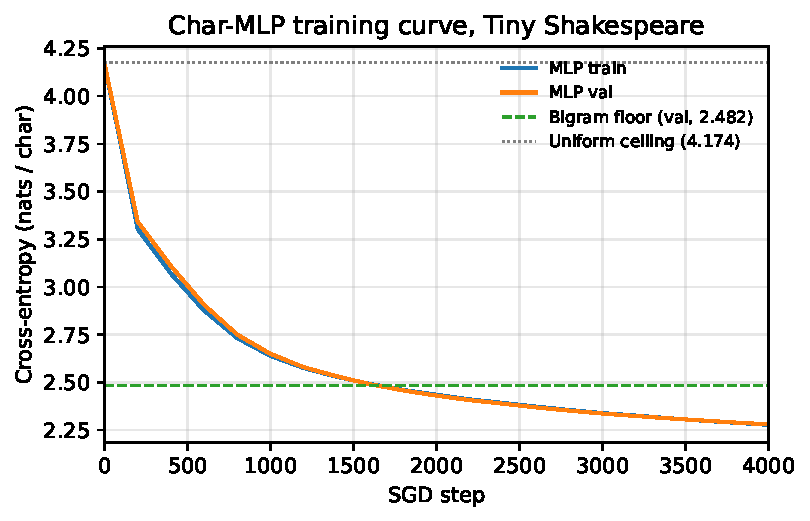
\includegraphics[width=\textwidth]{figures/training_curves.pdf}
    \captionof*{figure}{(a) MLP train+val CE vs.\ SGD step. Val crosses the bigram floor (dashed green) around step 1700.}
  \end{minipage}\hfill
  \begin{minipage}[t]{0.49\textwidth}
    \centering
    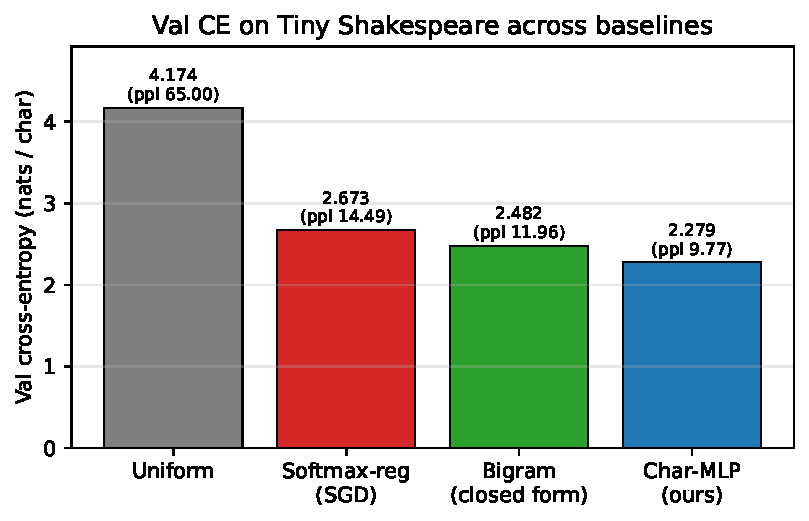
\includegraphics[width=\textwidth]{figures/baselines_comparison.pdf}
    \captionof*{figure}{(b) Val CE across the four reference points. Lower is better.}
  \end{minipage}
  \caption{Headline results from the engine and baselines.}
  \label{fig:headline}
\end{figure}

\subsection{Engine validation} Correctness, not raw performance, is the immediate concern: an undetected gradient bug invalidates every later experiment. We layered three checks:
\begin{itemize}
\setlength{\itemsep}{0pt}
  \item \textbf{Numerical gradient check} on every op individually (\textit{add}, \textit{mul}, \textit{div}, \textit{pow}, broadcast cases, reductions on every keepdims/axis combo, matmul on three batching patterns, gather with repeated indices, reshape, tanh, relu, log\_softmax, cross\_entropy). Tolerance \texttt{atol=1e-7, rtol=1e-5}; all 59 cases pass.
  \item \textbf{End-to-end gradcheck on the MLP forward pass}: gradient of the CE loss against all five parameter tensors (\texttt{E}, \texttt{W}$_1$, \texttt{b}$_1$, \texttt{W}$_2$, \texttt{b}$_2$) on randomized inputs.
  \item \textbf{PyTorch parity}: same MLP forward and backward computed in our engine and in \texttt{torch.autograd}; loss bit-identical, all five gradients within $5\!\times\!10^{-17}$ — below \texttt{float64} machine epsilon ($\sim\!2.2\!\times\!10^{-16}$).
\end{itemize}
The total project test suite has 103 passing cases.

\subsection{What the eval pipeline gives us for free} Because \texttt{full\_corpus\_ce} runs over every consecutive bigram pair (rather than a sampled subset), val CE is directly comparable across model classes — bigram counts, SGD-trained logits, and MLP forward all consume the same sequence and report the same mean over the same 111{,}539 positions. The $-0.20$-nat gap in Table~\ref{tab:results} reflects model class, not evaluation noise.

\section{Next Steps}

\begin{enumerate}
\setlength{\itemsep}{0pt}
  \item \textbf{Scaled-dot-product attention, forward and backward,} implemented in our engine using the closed-form Q/K/V projection Jacobians and the softmax-row identity already derived. The Tensor engine has matmul, log-softmax, and gather-shaped scatter, so the backward closures plug directly in. Verified by per-op gradcheck and parity against \texttt{torch.autograd}.
  \item \textbf{LayerNorm forward + backward,} validated by gradcheck and torch parity.
  \item \textbf{Decoder block} with toggleable LayerNorm placement (pre-norm / post-norm / none) and residual on/off — exactly the 6 configurations the ablation grid will sweep.
  \item \textbf{Ablation grid.} Train all 6 configs on Tiny Shakespeare, single seed, identical batches (the data layer's reproducible RNG was built for this). Per-step log: layer-wise $\Vert g \Vert_2$, activation norms, and the singular-value spectrum of layer Jacobians.
  \item \textbf{Comparison curves}: gradient-norm trajectories per config, training curves per config, val perplexity at convergence.
\end{enumerate}

\noindent The MLP result here is a sanity floor; the transformer ablation is the contribution.

\section{Team Contributions}

\begin{itemize}
\setlength{\itemsep}{0pt}
  \item \textbf{Manikanta Harsha Nadimpalli:} Tiny Shakespeare data pipeline (loader, tokenizer, batched sampler with reproducibility); three classical baselines (uniform, closed-form Laplace bigram, softmax-regression by SGD with hand-derived gradients); scalar reverse-mode autograd engine with numerical gradient check and PyTorch parity; tensor reverse-mode autograd engine (broadcasting, reductions, matmul, gather, reshape, activations, log-softmax, cross-entropy) with per-op numerical gradient checks and end-to-end PyTorch parity; char-MLP forward and training loop; results, figures, and this writeup.
  \item \textbf{Luis Blanco Hoyos:} Closed-form derivation of the scaled-dot-product attention backward (softmax-row Jacobian collapse, batched-matmul fan-in, three-path $X$ contribution, causal-mask handling); a PyTorch reference implementation for the forward pass and the closed-form backward; four \texttt{float64} parity tests at \texttt{1e-9} tolerance against \texttt{torch.autograd.grad}, with and without causal mask. This serves as the specification our autograd-engine attention will be built and verified against.
\end{itemize}

% References
{\footnotesize
\begin{thebibliography}{9}
\bibitem{vaswani2017attention} Vaswani, A., Shazeer, N., Parmar, N., Uszkoreit, J., Jones, L., Gomez, A.N., Kaiser, {\L}., Polosukhin, I. (2017). Attention is all you need. \textit{NeurIPS 30}.
\bibitem{karpathy2020micrograd} Karpathy, A. (2020). micrograd: A tiny scalar-valued autograd engine. \url{https://github.com/karpathy/micrograd}.
\bibitem{karpathy2015charrnn} Karpathy, A. (2015). The Unreasonable Effectiveness of Recurrent Neural Networks. \url{https://karpathy.github.io/2015/05/21/rnn-effectiveness/}.
\bibitem{ba2016layernorm} Ba, J.L., Kiros, J.R., Hinton, G.E. (2016). Layer Normalization. \textit{arXiv:1607.06450}.
\bibitem{bengio2003neural} Bengio, Y., Ducharme, R., Vincent, P., Jauvin, C. (2003). A Neural Probabilistic Language Model. \textit{JMLR 3}, 1137--1155.
\end{thebibliography}
}

\end{document}
